\documentclass[11pt]{article}
\usepackage[margin=1in]{geometry}
\usepackage{amsmath,amssymb}
\usepackage{graphicx}
\usepackage{hyperref}
\usepackage{parskip}

\title{Final Project:\\Multi-Exposure Modelling of Information Spread Through Social Media Reposting}
\author{Lavanya Kumar\\Student Number: 219148790}
\date{}

\begin{document}
\maketitle

\begin{abstract}
\noindent
We study how a single item of content spreads on social media when users may need repeated exposures before reposting or may disengage without sharing. A compartment model tracks exposure classes $I_0,\ldots,I_m$, active sharers $S$, and saturated users $R$, with mean-field exposure rate $\lambda=\beta S/N$. We relate the structure to classical rumor and complex-contagion literature, derive a reproduction-style threshold for $m=2$, analyze equilibria and local stability at the disease-free state, and run Python simulations for viral, moderate, and fizzle regimes. Sensitivity of peak sharing to $\beta$ and $\gamma$ is reported. We interpret results for Instagram-style repost dynamics and discuss limitations and extensions.
\end{abstract}

\section{Introduction}

Social platforms such as Instagram distribute content through feeds, recommendations, and reposting (Meta Platforms Inc., 2024). The same post can appear multiple times before a user reshares it, so \emph{exposure counts} matter, not only a binary ``seen / not seen'' label.

Classical information-diffusion models often use a fixed exposure threshold or a simple susceptible--infected--recovered (SIR) analogy. Real behaviour is heterogeneous: some users share after one view, others require reinforcement, and some lose interest. This project develops and analyzes an ordinary differential equation (ODE) model with \emph{multiple exposure classes} $I_i$ in which sharing or saturation can occur at any level $i\in\{0,\ldots,m\}$.

\textbf{Research questions.}
\begin{enumerate}
    \item Under what parameter conditions does reposting amplify from a small initial seed of sharers?
    \item How do repost intensity $\beta$ and attention decay $\gamma$ affect the peak number of active sharers and final reach?
    \item How can the same equations represent qualitatively different content (e.g.\ viral memes vs.\ slower news-like spread)?
\end{enumerate}

\section{Literature Review}

Rumor and information spread have long been modelled with epidemic-style compartments. Daley and Kendall (1965) introduced ignorants, spreaders, and stiflers; Maki and Thompson (1973) gave a related formulation. Kempe, Kleinberg, and Tardos (2003) studied influence maximization on networks. Centola (2010) showed experimentally that \emph{complex contagion} can require repeated exposure. Rogers (2003) described heterogeneous adoption timing across adopter types. Granovetter (1978) used threshold models where decisions depend on accumulated influence; our probabilities $(\rho_i,\sigma_i)$ play a similar role at each exposure stage.

The model below extends Daley--Kendall-type ideas with an explicit exposure chain $I_0\to\cdots\to I_m$, aligned with cumulative exposure on ranked feeds (Meta Platforms Inc., 2024).

\section{Model Formulation and Justification}

\subsection{Compartments and conservation}

Fix $N>0$. For $i=0,\ldots,m$, let $I_i(t)$ be the number of users who have been exposed exactly $i$ times and have not yet begun sharing the item. Let $S(t)$ be active sharers and $R(t)$ users who will not share further. Then
\begin{equation}
\sum_{i=0}^{m} I_i(t) + S(t) + R(t) = N.
\label{eq:cons}
\end{equation}
Table~\ref{tab:vars} lists symbols.

\subsection{Assumptions}

\begin{enumerate}
    \item The audience size $N$ is constant over the horizon.
    \item Mean-field mixing: exposure rate $\lambda(t)=\beta S(t)/N$, $\beta>0$.
    \item On each exposure while in $I_i$, the user shares with probability $\rho_i$, saturates with probability $\sigma_i$, or moves to $I_{i+1}$ with probability $1-\rho_i-\sigma_i$, with $0\le\rho_i,\sigma_i\le 1$ and $\rho_i+\sigma_i\le 1$.
    \item Sharers stop at rate $\gamma>0$.
    \item A single content item is studied (no competing posts).
\end{enumerate}

\subsection{Relation to fixed-threshold models}

If $\rho_i=\sigma_i=0$ for all $i<m$, users cannot leave the exposure chain until $I_m$; the next exposure forces sharing or saturation through $(\rho_m,\sigma_m)$. The general model therefore embeds a classical ``exactly $m$ exposures then decide'' rule as a special case.

\subsection{Governing equations}

With $\lambda(t)=\beta S(t)/N$,
\begin{align}
\frac{dI_0}{dt} &= -\lambda I_0, \label{eq:I0}\\
\frac{dI_i}{dt} &= (1-\rho_{i-1}-\sigma_{i-1})\lambda I_{i-1} - \lambda I_i, \quad i=1,\ldots,m-1, \label{eq:Ii}\\
\frac{dI_m}{dt} &= (1-\rho_{m-1}-\sigma_{m-1})\lambda I_{m-1} - (\rho_m+\sigma_m)\lambda I_m, \label{eq:Im}\\
\frac{dS}{dt} &= \sum_{i=0}^{m} \rho_i \lambda I_i - \gamma S, \label{eq:S}\\
\frac{dR}{dt} &= \sum_{i=0}^{m} \sigma_i \lambda I_i + \gamma S. \label{eq:R}
\end{align}
Equation~\eqref{eq:S} shows that $S$ grows when the inflow $\sum_i \rho_i\lambda I_i$ exceeds the outflow $\gamma S$. Summing \eqref{eq:I0}--\eqref{eq:R} confirms $d(I_0+\cdots+I_m+S+R)/dt=0$.

\begin{table}[htbp]
\centering
\caption{Model variables and parameters.}
\label{tab:vars}
\begin{tabular}{|l|l|}
\hline
\textbf{Symbol} & \textbf{Description} \\
\hline
$N$ & Total population \\
$m$ & Maximum exposure index \\
$I_i(t)$ & Exposed $i$ times, not yet sharing \\
$S(t)$ & Active sharers \\
$R(t)$ & Saturated users \\
$\beta$ & Repost intensity in $\lambda=\beta S/N$ \\
$\gamma$ & Sharer decay rate \\
$\rho_i,\sigma_i$ & Share / saturate probabilities at exposure $i$ \\
\hline
\end{tabular}
\end{table}

\section{Model Analysis}

\subsection{Reproduction-style threshold \texorpdfstring{($m=2$)}{(m = 2)}}

We use a scalar summary analogous to a basic reproduction number:
\begin{equation}
R_{\mathrm{eff}} \approx \frac{\beta}{\gamma}\,p_{\mathrm{share}},
\label{eq:Reff}
\end{equation}
where $p_{\mathrm{share}}$ approximates the probability that a user beginning in $I_0$ eventually enters $S$. For $m=2$,
\begin{equation}
p_{\mathrm{share}} \approx \rho_0 + (1-\rho_0-\sigma_0)\rho_1 + (1-\rho_0-\sigma_0)(1-\rho_1-\sigma_1)\rho_2.
\label{eq:pshare}
\end{equation}
Large $\beta$ or $\rho_i$ increases $R_{\mathrm{eff}}$; large $\gamma$ or $\sigma_i$ decreases it. We use $R_{\mathrm{eff}}$ to interpret simulation outcomes alongside the Jacobian below.

\subsection{Equilibria}

\paragraph{Disease-free equilibrium $E_0$.} $(I_0,I_1,\ldots,I_m,S)=(N,0,\ldots,0,0)$ and $R=0$. Here $\lambda=0$ and all time derivatives vanish: no exposures occur without sharers.

\paragraph{Absorbing equilibrium $E_\ast$.} $(I_0,\ldots,I_m,S)=(0,\ldots,0,0)$ and $R=N$. Again $\lambda=0$; the content has ``burned out'' and everyone is saturated. Simulations approach states near $E_\ast$ after large cascades.

\subsection{Local stability \texorpdfstring{at $E_0$ for $m=2$}{at E0 for m = 2}}

Let the state be $(I_0,I_1,I_2,S)$ with $R=N-I_0-I_1-I_2-S$. The Jacobian at $E_0$ (evaluate at $I_0=N$, $I_1=I_2=S=0$, $\lambda=0$) is
\begin{equation}
J(E_0)=
\begin{pmatrix}
0 & 0 & 0 & -\beta \\
0 & 0 & 0 & (1-\rho_0-\sigma_0)\beta \\
0 & 0 & 0 & 0 \\
0 & 0 & 0 & \rho_0\beta-\gamma
\end{pmatrix}.
\label{eq:Jac}
\end{equation}
Eigenvalues are $0$ (algebraic multiplicity three) and $\lambda_S=\rho_0\beta-\gamma$. The zero eigenvalues reflect the fact that when $\lambda=0$, the exposure chain is frozen until $S$ perturbs away from zero; the nonzero eigenvalue $\lambda_S$ governs the linearized growth or decay of $S$ in the direction tied directly to $I_0$. Secondary creation of sharers through $I_1,I_2$ appears once $\lambda>0$ and is captured by simulations and by $R_{\mathrm{eff}}$ in \eqref{eq:Reff}. Nonlinear global behaviour (large outbreaks) is therefore assessed numerically in \S\ref{sec:comp}.

\subsection{Computational methods}
\label{sec:comp}

We integrate \eqref{eq:I0}--\eqref{eq:R} with $m=2$ using Python~3 and \texttt{scipy.integrate.odeint} (see \path{simulate_instagram_ode.py}). Parameters use $N=1000$, initial condition $I_0(0)=985$, $I_1(0)=I_2(0)=0$, $S(0)=15$, $R(0)=0$, and $t\in[0,120]$ in dimensionless time units. Three labelled scenarios (viral, moderate, fizzle) are defined in Table~\ref{tab:param}.

\textbf{Figure files.} Place the generated PDFs in the same directory as this \texttt{.tex} file. Regenerate them with \texttt{python3}~\path{simulate_instagram_ode.py}. The manuscript embeds five PDFs, numbered Figure~1--5 below (Figure~1--3 trajectories; Figure~4--5 sensitivity).

\begin{table}[htbp]
\centering
\caption{Scenario parameters ($m=2$).}
\label{tab:param}
\begin{tabular}{|l|l|l|}
\hline
\textbf{Scenario} & $(\beta,\gamma)$ & $(\rho_0,\rho_1,\rho_2)$; $(\sigma_0,\sigma_1,\sigma_2)$ \\
\hline
Viral & (1.50, 0.080) & (0.05,0.15,0.25); (0.01,0.02,0.04) \\
Moderate & (1.13, 0.089) & same as viral \\
Fizzle & (0.15, 0.600) & (0.01,0.02,0.03); (0.10,0.15,0.20) \\
\hline
\end{tabular}
\end{table}

\begin{table}[htbp]
\centering
\caption{Numerical outcomes ($N=1000$, $S(0)=15$, $t\in[0,120]$).}
\label{tab:out}
\begin{tabular}{|l|c|c|c|c|}
\hline
\textbf{Scenario} & \textbf{Peak $S(t)$} & \textbf{Time to peak} & \textbf{$R(120)$} & \textbf{$p_{\mathrm{share}}$} \eqref{eq:pshare} \\
\hline
Viral & 321.66 & 51.29 & 981.56 & $\approx 0.34$ \\
Moderate & 171.51 & 114.39 & 593.46 & $\approx 0.34$ \\
Fizzle & 15.00 & 0.00 & 15.41 & $\approx 0.05$ \\
\hline
\end{tabular}
\end{table}

Table~\ref{tab:out} shows a clear ordering: viral and moderate share the same $p_{\mathrm{share}}$ but different $\beta/\gamma$, producing a much larger peak when $\beta/\gamma$ is higher; fizzle combines low $p_{\mathrm{share}}$ with low $\beta/\gamma$, so the seed does not ignite a cascade.

\subsection{Figures: simulation trajectories}

Figures~\ref{fig:vf}--\ref{fig:viralall} summarize trajectories. Viral runs show a large peak in $S(t)$ and most users ending in $R$; fizzle runs show $S(t)\approx S(0)$ and low $R$; moderate lies between.

\begin{figure}[htbp]
\centering
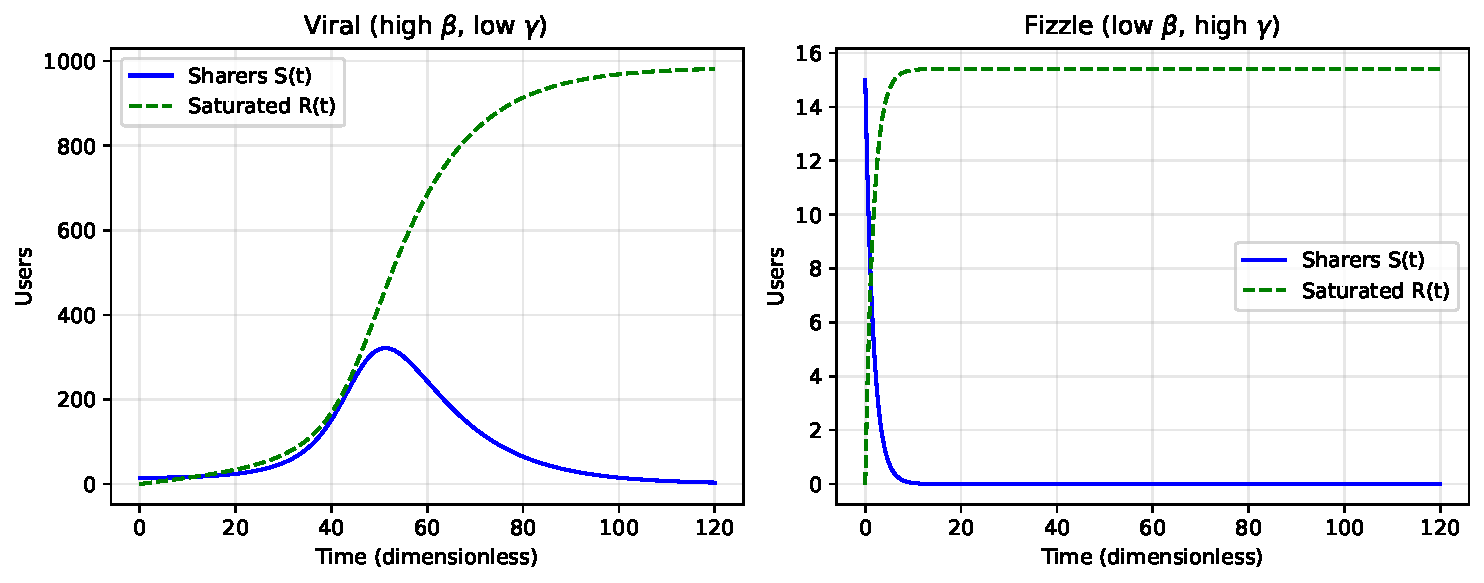
\includegraphics[width=0.95\textwidth]{fig_viral_vs_fizzle.pdf}
\caption{Viral (left) vs.\ fizzle (right): $S(t)$ and $R(t)$. \textit{File:} \texttt{fig\_viral\_vs\_fizzle.pdf}.}
\label{fig:vf}
\end{figure}

\begin{figure}[htbp]
\centering
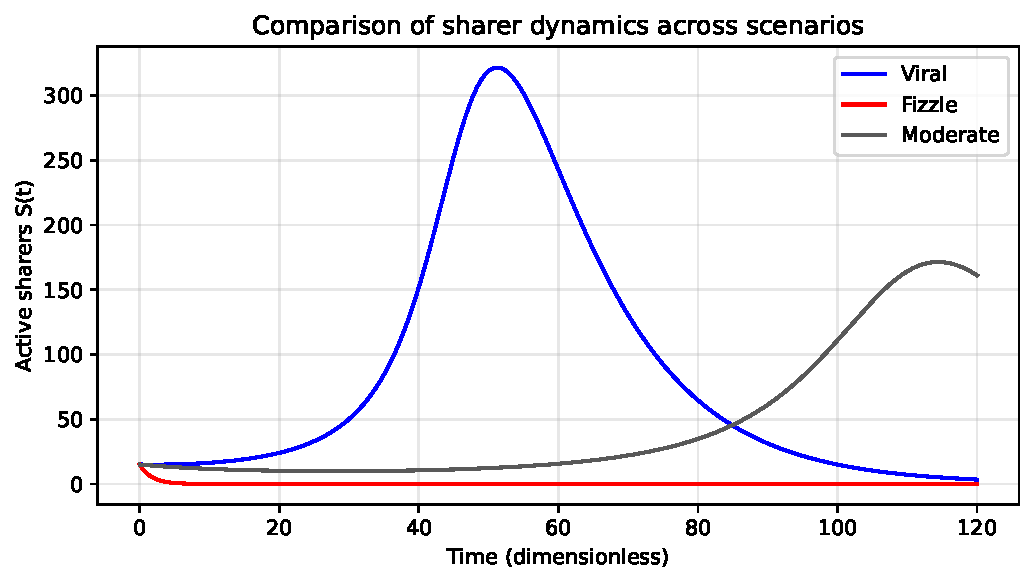
\includegraphics[width=0.75\textwidth]{fig_comparison.pdf}
\caption{Active sharers $S(t)$: viral, moderate, and fizzle. \textit{File:} \texttt{fig\_comparison.pdf}.}
\label{fig:cmp}
\end{figure}

\begin{figure}[htbp]
\centering
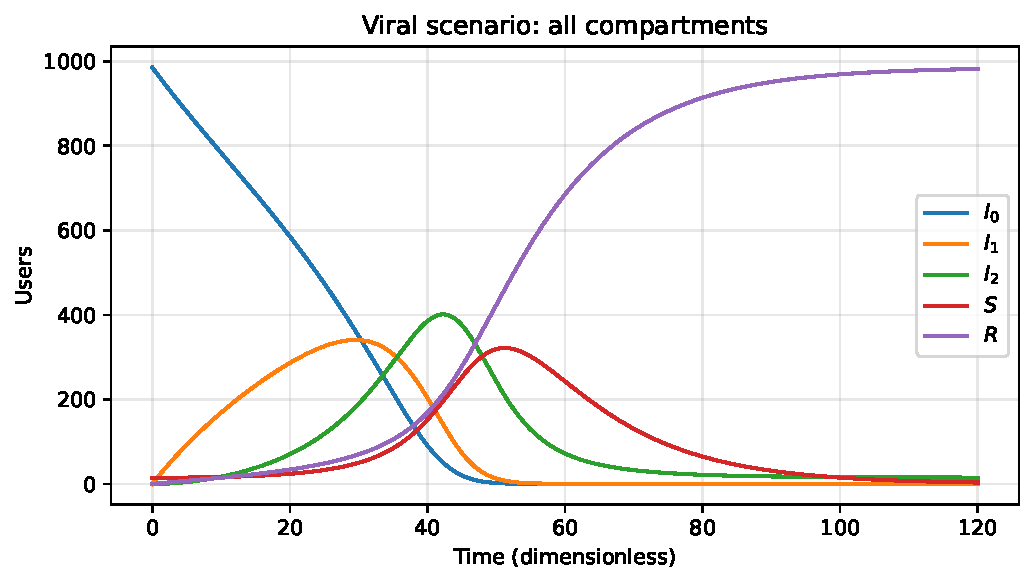
\includegraphics[width=0.75\textwidth]{fig_exposure_classes.pdf}
\caption{Viral scenario: all compartments over time. \textit{File:} \texttt{fig\_exposure\_classes.pdf}.}
\label{fig:viralall}
\end{figure}

\subsection{Sensitivity analysis}

Figure~\ref{fig:sensb} varies $\beta$ with fixed $\gamma=0.09$ and viral $(\rho_i,\sigma_i)$: peak $\max_t S(t)$ rises steeply once $\beta$ crosses a threshold band, consistent with \eqref{eq:Reff}. Figure~\ref{fig:sensg} varies $\gamma$ with fixed $\beta=1.2$: larger decay suppresses the peak, eventually collapsing it to the initial seed level.

\begin{table}[htbp]
\centering
\caption{Selected sensitivity values (same $N$, seed, and viral $(\rho_i,\sigma_i)$ as Table~\ref{tab:param}).}
\label{tab:sens}
\begin{tabular}{|l|c|c|}
\hline
\textbf{Vary $\beta$} ($\gamma=0.09$) & $\beta$ & Peak $S(t)$ \\
\hline
 & 0.5 & 15.0 \\
 & 1.0 & 15.0 \\
 & 1.5 & 278.6 \\
\hline
\textbf{Vary $\gamma$} ($\beta=1.2$) & $\gamma$ & Peak $S(t)$ \\
\hline
 & 0.08 & 238.3 \\
 & 0.12 & 15.0 \\
 & 0.20 & 15.0 \\
\hline
\end{tabular}
\end{table}

\begin{figure}[htbp]
\centering
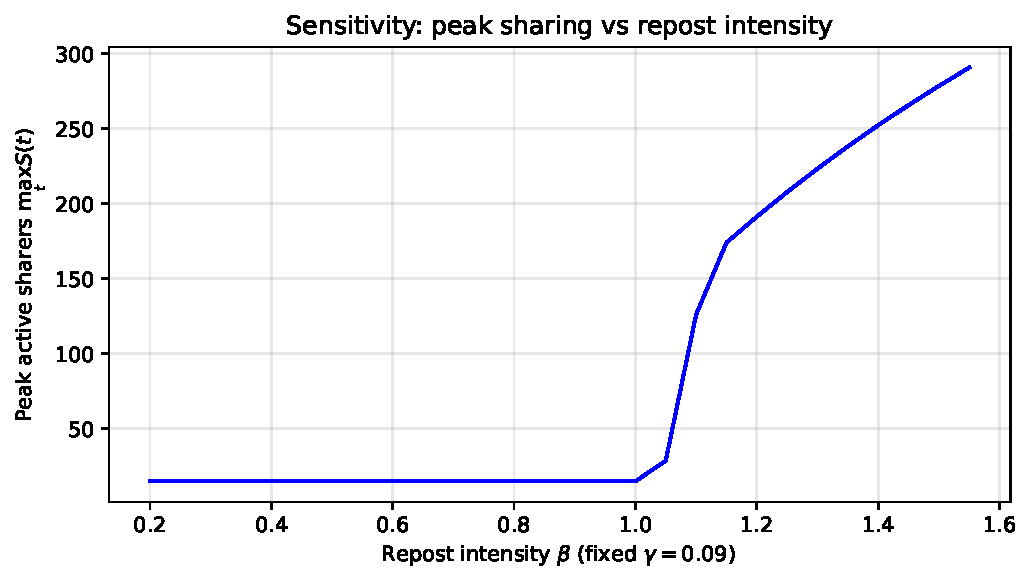
\includegraphics[width=0.75\textwidth]{fig_sensitivity_beta.pdf}
\caption{Peak $\max_t S(t)$ vs.\ $\beta$ ($\gamma=0.09$, viral probabilities). \textit{File:} \texttt{fig\_sensitivity\_beta.pdf}.}
\label{fig:sensb}
\end{figure}

\begin{figure}[htbp]
\centering
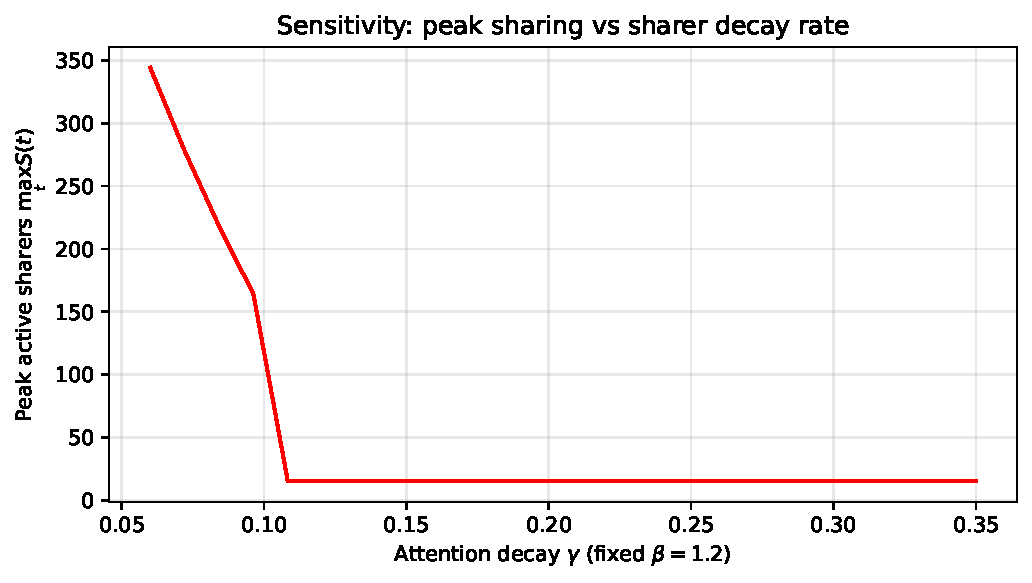
\includegraphics[width=0.75\textwidth]{fig_sensitivity_gamma.pdf}
\caption{Peak $\max_t S(t)$ vs.\ $\gamma$ ($\beta=1.2$, viral probabilities). \textit{File:} \texttt{fig\_sensitivity\_gamma.pdf}.}
\label{fig:sensg}
\end{figure}

\subsection{Interpretation for social media}

High $\beta$ (strong resharing visibility) and low $\gamma$ (slow loss of interest among sharers) promote large cascades, matching intuition for viral memes. Reducing $\beta/\gamma$ yields moderate peaks---content that spreads but does not explode. High $\gamma$, low $\beta$, or high loss probabilities $\sigma_i$ produce fizzle, analogous to low-engagement posts. The exposure classes $I_0,I_1,I_2$ formalize reinforcement before sharing (Centola, 2010).

\section{Discussion and Conclusions}

We formulated a multi-exposure ODE model for repost-driven spread, connected it to rumor and complex-contagion literature, and analyzed a reproduction-style quantity $R_{\mathrm{eff}}$ for $m=2$. Local linearization at the disease-free equilibrium yields the Jacobian \eqref{eq:Jac}, highlighting degeneracy at $\lambda=0$ and the eigenvalue $\rho_0\beta-\gamma$ for the sharer direction. Python simulations distinguish viral, moderate, and fizzle regimes and show sensitivity of peak sharing to $\beta$ and $\gamma$.

\textbf{Strengths.} The model is interpretable, conserves $N$, generalizes a fixed-threshold special case, and produces clear comparative statics aligned with platform intuition.

\textbf{Limitations and drawbacks.} Homogeneous mixing ignores follower-network structure (Kempe et al., 2003). Parameters are illustrative, not estimated from data. The Jacobian analysis at $E_0$ does not by itself rule in or out large nonlinear outbreaks driven by the $I_1,I_2$ chain; we relied on simulation for global behaviour.

\textbf{Extensions that would add knowledge.} Degree-weighted exposure or a small network toy model; estimation of $(\beta,\gamma,\rho_i,\sigma_i)$ from engagement time series; multiple competing items; stochastic simulations to capture discrete repost events.

\section{References}

Centola, D. (2010). The spread of behavior in an online social network experiment. \textit{Science}, 329(5996), 1194--1197.

Daley, D. J., \& Kendall, D. G. (1965). Stochastic rumours. \textit{Journal of the Institute of Mathematics and its Applications}, 1(1), 42--55.

Granovetter, M. (1978). Threshold models of collective behavior. \textit{American Journal of Sociology}, 83(6), 1420--1443.

Kempe, D., Kleinberg, J., \& Tardos, \'{E}. (2003). Maximizing the spread of influence through a social network. In \textit{Proceedings of the Ninth ACM SIGKDD International Conference on Knowledge Discovery and Data Mining} (pp.~137--146).

Maki, D. P., \& Thompson, M. (1973). \textit{Mathematical Models and Applications: With Emphasis on the Social, Life, and Management Sciences}. Prentice Hall.

Meta Platforms Inc. (2024). How the Instagram algorithm works. Instagram Help Center. Retrieved from \url{https://help.instagram.com/}

Rogers, E. M. (2003). \textit{Diffusion of Innovations} (5th ed.). New York: Free Press.

\end{document}
